\section{Research Data Management
101}\label{research-data-management-101}

\subsection{Michelle Hudson}\label{michelle-hudson}

\subsubsection{CSSSI StatLab workshop Oct 14
2016}\label{csssi-statlab-workshop-oct-14-2016}

\subparagraph{\texorpdfstring{\url{https://github.com/michellehudson/datamanagement}}{https://github.com/michellehudson/datamanagement}}\label{httpsgithub.commichellehudsondatamanagement}

\section{Description:}\label{description}

This two-hour workshop will provide an overview of the data lifecycle
and the critical steps within it that need to be addressed to ensure
integrity of research data. It is appropriate for students and faculty
in all disciplines, however, the constrained time-frame and high level
overview of the issues only warrant a few in-depth examples of tools and
resources for specific disciplines. The workshop will focus on general
good practices for data management that span disciplines. There will be
Q\&A time for specific questions, and attendees are always welcome to
follow up with instructors or other specialist for more tailored data
management instruction or assistance.

\section{Data lifecycle model}\label{data-lifecycle-model}

\begin{figure}[htbp]
\centering
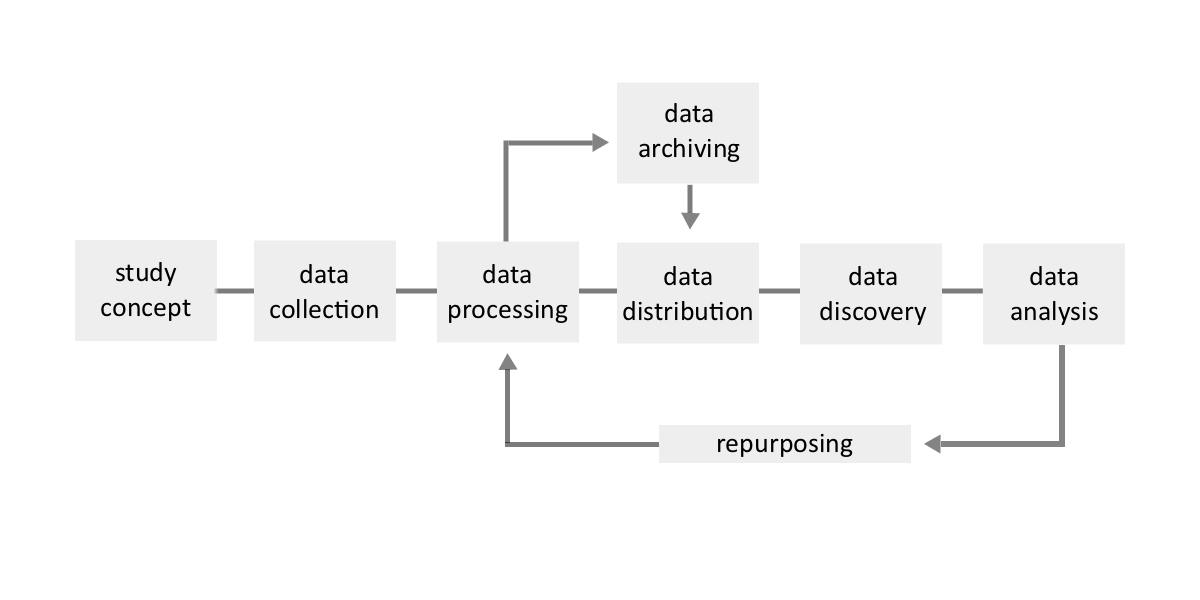
\includegraphics{https://raw.githubusercontent.com/michellehudson/datamanagement/master/research_data_management_101/2016_fall/images/ddilifecycle.png}
\caption{DDI lifecycle model}
\end{figure}

\section{Outline:}\label{outline}

\begin{enumerate}
\def\labelenumi{\arabic{enumi}.}
\tightlist
\item
  Research Data Consultation Group
\item
  What is data?
\item
  Why manage it?
\item
  Data management checklist
\item
  Data Management Planning
\item
  Metadata and data description
\item
  Organizing and working with data files
\item
  Re-using data and making your data reusable
\item
  Storage, computing, and analysis
\item
  Data preservation and archiving data
\item
  Sharing and publishing data
\item
  Resources list
\end{enumerate}

\section{Research Data Consultation
Group}\label{research-data-consultation-group}

\href{http://researchdata.yale.edu/}{http://researchdata.yale.edu}

RDCG has 13 consultants from across Yale to help consult on finding and
using data, analyzing data, storage options, preserving and archiving
data, and more. Use the
\href{http://researchdata.yale.edu/contact}{contact form} at
\href{http://researchdata.yale.edu/}{http://researchdata.yale.edu} to
get assistance with research data issues at any point in your project.

\section{What is research data?}\label{what-is-research-data}

Research data is defined as ``the recorded factual material commonly
accepted in the scientific community as necessary to validate research
findings.'' - OMB Circular A-110. More loosely, it's defined as
\emph{information collected, observed, or created for purposes of
analysis to produce original research.}

There are four general types of research data:

\begin{enumerate}
\def\labelenumi{\arabic{enumi}.}
\tightlist
\item
  Observational: captured in real time, usually irreplaceable (sensor
  readings, telescope images, sample data, surveys).
\item
  Experimental: data from lab equipment, can be reproducible but may be
  expensive (gene sequences).
\item
  Simulation: data generated from test models (climate models).
\item
  Derived or compiled: reproducible but expensive (data mining, compiled
  databases).
\end{enumerate}

Research data comes in many formats of information: documents,
spreadsheets, field notebooks, survey responses, audio and video
recordings, images, film, specimens, software code, and can be
structured and stored in a variety of file formats.

\section{Why manage research data?}\label{why-manage-research-data}

There are many reasons why good data management is important for your
research career, ranging from long-term effects on the future of science
to personal productivity and accomplishment.

\subsection{Transparency, integrity, and
reproducibility:}\label{transparency-integrity-and-reproducibility}

Managing data and making it accessible by peers decreases the chances of
an article being retracted because of falsified or missing data sets.
Reproducibility is a fundamental part of scientific research, and
failing to make all the components of a research study available makes
reproducibility impossible.

\subsection{Compliance:}\label{compliance}

Data management plans are required by funding agencies, and there is
increased expectation that the products of federal funding will be
required to be accessible to the public. See more information about this
on the
\href{https://www.whitehouse.gov/blog/2013/02/22/expanding-public-access-results-federally-funded-research}{whitehouse.gov
post on the OSTP Memo on Expanding Public Access to the Results of
Federally Funded Research}. In addition, many journals are requiring
data deposit before an article may be published.

\subsection{Personal \& professional
benefits:}\label{personal-professional-benefits}

If data is managed within your lab, research group, or simply
well-organized for your own use, you will save time, energy, and
resources. All members of the team will have an understanding of the
well-documented processing and analysis of the project's data, and be
able to carry out their research components more effectively. Sharing
research data is now regarded as an integral and valuable part of the
research process, and archiving your data in a repository will allow
other researchers to build upon your work and cite you in the process.

\section{Data management checklist}\label{data-management-checklist}

\begin{enumerate}
\def\labelenumi{\arabic{enumi}.}
\tightlist
\item
  always keep original data
\item
  back up regularly\\
\item
  document your data thoroughly
\item
  name and organize files according to a schema
\item
  use version control
\item
  secure the data appropriately
\item
  cite any secondary data you use
\item
  consider your long-term plan: What will you keep, for how long, where,
  and who will pay for it? What kinds of reuse or sharing will be
  allowed? In what timeframe?
\end{enumerate}

\section{Data Management Planning}\label{data-management-planning}

\subsection{What is a DMP?}\label{what-is-a-dmp}

Some funding agencies require a short document called a Data Management
Plan that supplements a grant proposal and explains how data will be
managed throughout a project, who will be responsible for managing it,
and how it will be shared when the project ends.

\subsection{Which agencies require a
DMP?}\label{which-agencies-require-a-dmp}

All NSF directorates, the NIH, and several other smaller funding
agencies require a formal data management plan to be submitted with
proposals. In addition, every federal agency that receives more than 100
million in R\&D expenditures has been instructed to develop plans to
require researchers to ``better account for and manage the digital data
resulting from federally funded scientific research.'' -
\href{https://www.whitehouse.gov/blog/2013/02/22/expanding-public-access-results-federally-funded-research}{OSTP}.
Many of the agencies have responded by requiring DMPs. You can find a
list of all the agencies and their guidelines at
\href{http://datasharing.sparcopen.org}{SPARC}.

\subsection{What tools and resources are available to help me write a
DMP?}\label{what-tools-and-resources-are-available-to-help-me-write-a-dmp}

\paragraph{\texorpdfstring{DMPTool:
\href{https://dmptool.org/}{https://dmptool.org}:}{DMPTool: https://dmptool.org:}}\label{dmptool-httpsdmptool.org}

Yale is a DMPTool partner. Logging in with your Yale ID and password
will give you access to the DMPTool, which will give you an overview of
funder requirements (for various NSF, NIH, and other directorates and
divisions), and walk you through building a data management plan, asking
the right questions along the way.

\paragraph{\texorpdfstring{Research Data Consultation Group:
\url{http://researchdata.yale.edu/contact}:}{Research Data Consultation Group: http://researchdata.yale.edu/contact:}}\label{research-data-consultation-group-httpresearchdata.yale.educontact}

If you have to submit a DMP as part of a grant proposal and have trouble
using the DMPTool or answering questions you think are critical to the
good management of data, you can contact the Research Data Consultation
Group for help. This group can review written plans and offer feedback,
or connect you with more resources at Yale you might be able to cite or
consider including in your plan to make a stronger proposal.

\paragraph{\texorpdfstring{StatLab consultants:
\url{http://csssi.yale.edu/data/csssi-statistical-consulting}:}{StatLab consultants: http://csssi.yale.edu/data/csssi-statistical-consulting:}}\label{statlab-consultants-httpcsssi.yale.edudatacsssi-statistical-consulting}

Even if you aren't submitting a grant proposal, it's a good idea to come
to the StatLab at the beginning of your project. If you know what
analyses you want to do on your data, the StatLab can make sure you set
out to collect your data correctly. If you anticipate using StatLab
services near the end of your project, it's much easier for them if you
connect in the beginning of the project, as well.

\subsection{Things to consider when writing a
DMP}\label{things-to-consider-when-writing-a-dmp}

\begin{itemize}
\tightlist
\item
  What data are generated by your research?

  \begin{itemize}
  \tightlist
  \item
    Describe intended file formats, instruments and software used,
    collection notes, collection materials (surveys or tests), metadata
    standards applied
  \end{itemize}
\item
  What is your plan for managing the data?

  \begin{itemize}
  \tightlist
  \item
    How will the data be stored while the project is in progress?
  \item
    What security measures are necessary, if any?
  \item
    Who will be responsible for managing the data generated for the
    project, during and after?
  \item
    How will data be disseminated or shared after the project, and in
    what timeframe, under what conditions?
  \item
    Are there any limitations that you need to address re: personally
    identifiable or health information?
  \item
    How will necessary data be archived and preserved?
  \end{itemize}
\end{itemize}

\section{Metadata and data
description}\label{metadata-and-data-description}

\subsection{Metadata}\label{metadata}

Metadata is the ``data about data'' that is needed to make numeric data
usable. Without proper metadata and documentation of the research
methods, analysis, variables, units, codes, and locations relevant to
the numeric information, digital data is unusable.

\subsection{Types of metadata}\label{types-of-metadata}

\subsubsection{Descriptive}\label{descriptive}

Title, author, abstract, keywords, geographic coordinates,
species\ldots{}

\subsubsection{Structural}\label{structural}

Schematic relationships between files, relational information\ldots{}

\subsubsection{Administrative}\label{administrative}

Formats of data files, intellectual property information, preservation
metadata\ldots{}

\subsection{Levels of metadata}\label{levels-of-metadata}

\subsubsection{Study-level description}\label{study-level-description}

\begin{enumerate}
\def\labelenumi{\arabic{enumi}.}
\tightlist
\item
  Context of the data collection (project history, aim, objectives, and
  hypotheses)
\item
  Data collection methods (sampling, data collection process,
  instruments used, hardware and software used to collect data, scale
  and resolution, temporal and geographic coverage, secondary data
  sources used, if any)
\item
  Data set structure -- of files, study cases, and relationships between
  files
\item
  Changes made to data over time
\item
  Information on access and use conditions or data confidentiality
\end{enumerate}

\subsubsection{File-level description}\label{file-level-description}

\begin{enumerate}
\def\labelenumi{\arabic{enumi}.}
\tightlist
\item
  Names, labels, and descriptions for variables, records, and their
  values
\item
  Definition of codes \& classification schemes used
\item
  Codes of and reasons for missing values
\end{enumerate}

\subsubsection{Variable-level
description}\label{variable-level-description}

\begin{enumerate}
\def\labelenumi{\arabic{enumi}.}
\tightlist
\item
  What does each variable mean in the context of the research?
\end{enumerate}

\subsection{Examples of metadata
standards}\label{examples-of-metadata-standards}

\paragraph{\texorpdfstring{Data Documentation Initiative:
\href{http://www.ddialliance.org/}{http://www.ddialliance.org}}{Data Documentation Initiative: http://www.ddialliance.org}}\label{data-documentation-initiative-httpwww.ddialliance.org}

A freely available, international standard for describing statistical
and social science data.

\paragraph{\texorpdfstring{Ecological Markup Language:
\url{https://knb.ecoinformatics.org/\#external//emlparser/docs/index.html}}{Ecological Markup Language: https://knb.ecoinformatics.org/\#external//emlparser/docs/index.html}}\label{ecological-markup-language-httpsknb.ecoinformatics.orgexternalemlparserdocsindex.html}

The EML project is an open source, community oriented project dedicated
to providing a high-quality metadata specification for describing data
relevant to the ecological discipline.

\paragraph{\texorpdfstring{Darwin Core:
\url{http://rs.tdwg.org/dwc/}}{Darwin Core: http://rs.tdwg.org/dwc/}}\label{darwin-core-httprs.tdwg.orgdwc}

The Darwin Core is body of standards. It includes a glossary of terms
(in other contexts these might be called properties, elements, fields,
columns, attributes, or concepts) intended to facilitate the sharing of
information about biological diversity by providing reference
definitions, examples, and commentaries.

\paragraph{\texorpdfstring{ISO Geospatial Metadata Standards:
\url{https://www.fgdc.gov/metadata}}{ISO Geospatial Metadata Standards: https://www.fgdc.gov/metadata}}\label{iso-geospatial-metadata-standards-httpswww.fgdc.govmetadata}

Guides from the Federal Geographic Data Committee on applying
appropriate metadata to geospatial information.

\paragraph{\texorpdfstring{More:
\href{http://rd-alliance.github.io/metadata-directory/}{list of metadata
standards from the Research Data
Alliance}}{More: list of metadata standards from the Research Data Alliance}}\label{more-list-of-metadata-standards-from-the-research-data-alliance}

\subsection{What tools and resources are
available?}\label{what-tools-and-resources-are-available}

\paragraph{\texorpdfstring{Morpho:
\url{https://knb.ecoinformatics.org/morphoportal.jsp}}{Morpho: https://knb.ecoinformatics.org/morphoportal.jsp}}\label{morpho-httpsknb.ecoinformatics.orgmorphoportal.jsp}

Morpho was developed for data management in ecology.

\paragraph{\texorpdfstring{Colectica:
\href{http://www.colectica.com/}{http://www.colectica.com}}{Colectica: http://www.colectica.com}}\label{colectica-httpwww.colectica.com}

Colectica is software that helps design, document, and publish
statistical data and survey research using open data standards.

\paragraph{\texorpdfstring{ISO geospatial metadata editors:
\url{https://www.fgdc.gov/iso-metadata-editors-registry/editors}}{ISO geospatial metadata editors: https://www.fgdc.gov/iso-metadata-editors-registry/editors}}\label{iso-geospatial-metadata-editors-httpswww.fgdc.goviso-metadata-editors-registryeditors}

A comparison of tools available for editing geographic metadata.

\paragraph{\texorpdfstring{More:
\href{http://rd-alliance.github.io/metadata-directory/tools}{list of
metadata tools from the Research Data
Alliance}}{More: list of metadata tools from the Research Data Alliance}}\label{more-list-of-metadata-tools-from-the-research-data-alliance}

\subsection{Reminder!}\label{reminder}

\begin{figure}[htbp]
\centering
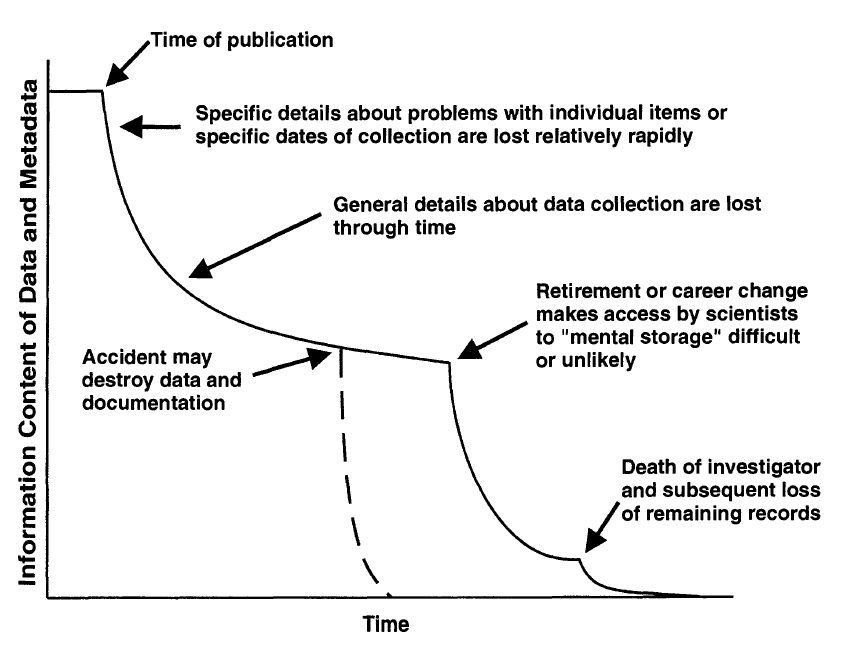
\includegraphics{https://raw.githubusercontent.com/michellehudson/datamanagement/master/research_data_management_101/2016_fall/images/death.png}
\caption{Bill Michener's description of data completeness over time}
\end{figure}

\section{Organizing and working with data
files}\label{organizing-and-working-with-data-files}

\subsection{Main takeaways}\label{main-takeaways}

\begin{enumerate}
\def\labelenumi{\arabic{enumi}.}
\tightlist
\item
  Keep a codebook for all data
\item
  Keep a log of all transforms and analyses (syntax)
\item
  Save data often and back up files
\item
  Use a versioning system
\item
  Organize files
\end{enumerate}

\subsection{Codebooks}\label{codebooks}

Codebooks are used in social science research to serve as a companion to
the numeric data -- a human-readable manual containing all the metadata
needed to understand and use data related to a project. You should have
a codebook for your project that explains each variable and its values,
any variables you've added or computed, etc.

Example: \href{http://gss.norc.org/Get-Documentation}{General Social
Survey codebook, 1972 - 2014}

In addition to creating a codebook, you can also create a readme.txt
file that lives in the home directory for your project and explains the
latest notes, updates, and reminders for your project's data files.

\subsection{Working with syntax files}\label{working-with-syntax-files}

Syntax files are separate text files used to enter commands that are
then performed on the data. Keeping a log of your analyses this way
makes your research more reliable (you can share your syntax code along
with your data sets for replication purposes). With syntax files, you
can add comments to commands so you remember why you performed which
actions.

The \href{http://isps.yale.edu/research/data}{ISPS Data Archive} keeps
data and syntax files for all studies. Example: Butler, Daniel M. et al.
(2015) Replication Materials for `Ideology, Learning and Policy
Diffusion: Experimental Evidence.'
\url{http://hdl.handle.net/10079/1zcrjs8}.'' ISPS Data Archive.

\subsection{Backup and versioning}\label{backup-and-versioning}

\begin{enumerate}
\def\labelenumi{\arabic{enumi}.}
\tightlist
\item
  Implement a system for backing up all your project-related files (Box,
  USB drives, network shares).
\item
  If you can't automate a system, back up manually according to a
  schedule and stick to it.
\item
  Explore options for using version tracking for data files, especially
  if more than one person is working on the same project.
\end{enumerate}

\subsection{Organize files and
folders}\label{organize-files-and-folders}

Before you begin a project, decide (in cooperation with your lab, PI, or
others if necessary) on a folder structure and naming convention. There
are few best practices around this during the active stage of working
with data, and researchers do it differently according to the needs of
their lab and their data. The best advice is to decide on something and
stick with it.

\subsubsection{Folder structure}\label{folder-structure}

\begin{itemize}
\tightlist
\item
  Use a hierarchical structure.
\item
  Keep original data and working files separate.
\item
  Keep a readme.txt.
\item
  Keep any geospatial data together in its folders.
\end{itemize}

\subsubsection{Folder structure example}\label{folder-structure-example}

\begin{figure}[htbp]
\centering
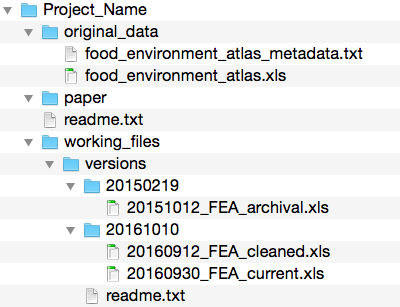
\includegraphics{https://raw.githubusercontent.com/michellehudson/datamanagement/master/research_data_management_101/2016_fall/images/folder_structure.png}
\caption{Example folder structure}
\end{figure}

\url{https://github.com/michellehudson/datamanagement/tree/master/research_data_management_101/2016_fall/ex_folder_structure}

\subsubsection{File naming}\label{file-naming}

\begin{itemize}
\tightlist
\item
  Use descriptive filenames, but not too long.
\item
  Do not use special characters.
\item
  Include date information at the beginning or end of the file and be
  consistent.
\item
  Use underscores, not spaces.
\item
  Considering including: project name, researcher initials, version
  number.
\end{itemize}

\subsubsection{File naming example}\label{file-naming-example}

\begin{figure}[htbp]
\centering
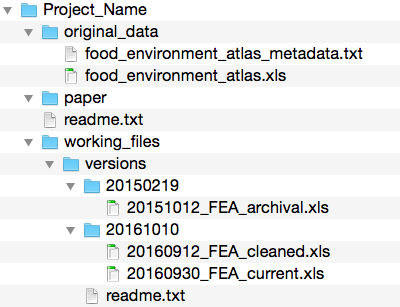
\includegraphics{https://raw.githubusercontent.com/michellehudson/datamanagement/master/research_data_management_101/2016_fall/images/folder_structure.png}
\caption{Example folder structure}
\end{figure}

\url{https://github.com/michellehudson/datamanagement/tree/master/research_data_management_101/2016_fall/ex_folder_structure}

\section{Re-using data and making your data
re-usable}\label{re-using-data-and-making-your-data-re-usable}

If you're re-using data from another source (downloaded from another
institute, a data archive, from another researcher, etc.), you want to
get to know it as completely as possible. If you're providing your data
to an archive or to another researcher so they can re-use it, think
about what information you'd need if you were using someone else's data,
and make sure that information is included for your own.

\begin{enumerate}
\def\labelenumi{\arabic{enumi}.}
\tightlist
\item
  How was the data collected? What instruments (survey or scientific)
  were used? If it was a survey, what was the wording of the questions?
  Who coded the questions?
\item
  How is the data coded? What are the codes for missing values, and what
  do they mean?
\item
  Is the data pre-processed or cleaned? Is it weighted? Are any values
  interpolated?
\end{enumerate}

\subsection{Finding data for re-use}\label{finding-data-for-re-use}

Librarians have created guides to assist with finding data in different
disciplines.

\begin{itemize}
\tightlist
\item
  \href{http://guides.library.yale.edu/data-statistics}{Social science
  data \& statistics}
\item
  \href{http://guides.library.yale.edu/sciencedata}{Science data}
\end{itemize}

Or, feel free to \href{http://bit.ly/meetmichellehudson}{schedule a
meeting with the data librarian} to discuss finding data for a project.

\section{Storage, computing, and
analysis}\label{storage-computing-and-analysis}

\subsection{Data storage}\label{data-storage}

\begin{itemize}
\tightlist
\item
  \href{http://its.yale.edu/services/email-and-collaboration-services/document-sharing-and-team-sites/box-yale}{Box}
\item
  \href{http://its.yale.edu/services/email-and-collaboration-services/document-sharing-and-team-sites/storageyale}{Storage@Yale}
\end{itemize}

\subsection{Computing}\label{computing}

\begin{itemize}
\item
  \href{http://research.computing.yale.edu/}{Yale Center for Research
  Computing} for HPC support and training
\item
  StatLab windows server for smaller jobs (talk to Themba Flowers for
  access)
\end{itemize}

\subsection{Data analysis}\label{data-analysis}

\begin{itemize}
\tightlist
\item
  \href{http://csssi.yale.edu/data-and-gis/csssi-statisical-consulting/csssi-statistical-and-gis-consultants}{StatLab
  consultants}
\item
  \href{http://csssi.yale.edu/instruction/workshop-and-instruction-calendar}{StatLab
  workshops}
\end{itemize}

\section{Preservation and archiving}\label{preservation-and-archiving}

Archiving and preserving research data is different from distributing it
or backing it up regularly. Preservation ensures long-term retention of
the data and the necessary migration from format to format that will be
required to keep the data usable over a time period. How long you retain
your data is often up to what your funding dictates -- some grants say
three years, others five. In some cases, your data may have value for an
indefinite period of time.

\subsection{Available repositories:}\label{available-repositories}

The Registry of Research Data Repositories \url{http://www.re3data.org}
aims to list all the data repositories available for submission or for
finding research data to reuse, and you can search or browse by subject.

\subsection{Guidelines:}\label{guidelines}

\begin{enumerate}
\def\labelenumi{\arabic{enumi}.}
\tightlist
\item
  Doing preservation yourself requires format migration and ensuring
  integrity of files.
\item
  Handing over your data to a repository like ICPSR is possible, and
  will ensure the data is usable over the long-term.
\end{enumerate}

\subsection{Examples:}\label{examples}

\paragraph{\texorpdfstring{Institution for Social \& Policy Studies:
\url{http://isps.yale.edu/research/data}}{Institution for Social \& Policy Studies: http://isps.yale.edu/research/data}}\label{institution-for-social-policy-studies-httpisps.yale.eduresearchdata}

ISPS is a Yale department that maintains a data archive of research that
has been conducted by their affiliates.

\paragraph{\texorpdfstring{ICPSR:
\url{http://icpsr.umich.edu}}{ICPSR: http://icpsr.umich.edu}}\label{icpsr-httpicpsr.umich.edu}

The Inter-university Consortium for Political and Social research is a
domain archive that has been curating and maintaining access to data
sets for over 50 years.

\section{Data sharing and publishing}\label{data-sharing-and-publishing}

\subsection{Platforms}\label{platforms}

There are many platforms for data distribution that are easy, free, and
meet many researcher needs. These solutions do not necessarily guarantee
preservation-level archiving for research data, but they make data
available and citable.

\subsubsection{\texorpdfstring{openICPSR:
\href{https://www.openicpsr.org/openicpsr/}{https://www.openicpsr.org}}{openICPSR: https://www.openicpsr.org}}\label{openicpsr-httpswww.openicpsr.org}

openICPSR is a branch of the ICPSR and is free for Yale researchers
depositing social science and behavioral health related datasets.

\subsubsection{\texorpdfstring{Open Science Framework:
\href{https://osf.io/}{https://osf.io}}{Open Science Framework: https://osf.io}}\label{open-science-framework-httpsosf.io}

The Open Science Framework is funded by federal agencies, private
foundations, and commercial entities, and offers a free platform for
data management and publication.

\subsubsection{\texorpdfstring{Dataverse:
\href{https://dataverse.harvard.edu/}{https://dataverse.harvard.edu}}{Dataverse: https://dataverse.harvard.edu}}\label{dataverse-httpsdataverse.harvard.edu}

Dataverse is repository software that institutions can set up and host,
but it's also a network of these repository nodes. The Harvard instance
of Dataverse is open to all researchers for data submission and
publication through a personal account.

\subsection{Data citation}\label{data-citation}

It's important for your data to be citable, and it's important to cite
any data you use in your analyses thoroughly. Look for a data sharing
platform that will give you a permanent identifier (like a DOI or a
handle) for your project.

DataCite \url{https://www.datacite.org/index.html} is an international
organization that provides permanent identifiers for data, and they
provide a helpful \href{https://www.datacite.org/citation.html}{citation
formatter for data}.

\section{Resources}\label{resources}

\paragraph{\texorpdfstring{Data Management Research Guide:
\url{http://guides.library.yale.edu/datamanagement}}{Data Management Research Guide: http://guides.library.yale.edu/datamanagement}}\label{data-management-research-guide-httpguides.library.yale.edudatamanagement}

CSSSI's data management guide.

\paragraph{\texorpdfstring{MANTRA:
\href{http://datalib.edina.ac.uk/mantra/}{http://datalib.edina.ac.uk/mantra}}{MANTRA: http://datalib.edina.ac.uk/mantra}}\label{mantra-httpdatalib.edina.ac.ukmantra}

Mantra is series of useful research data management training modules you
can complete online.

\section{Contact info}\label{contact-info}

\subsubsection{Michelle Hudson}\label{michelle-hudson-1}

\begin{itemize}
\tightlist
\item
  Science and Social Science Data Librarian
\item
  \href{mailto:michelle.hudson@yale.edu}{\nolinkurl{michelle.hudson@yale.edu}}
\end{itemize}

\subsubsection{Joshua Dull}\label{joshua-dull}

\begin{itemize}
\tightlist
\item
  Research Data Support Specialist
\item
  \href{mailto:joshua.dull@yale.edu}{\nolinkurl{joshua.dull@yale.edu}}
\end{itemize}

\subsubsection{StatLab Consultants}\label{statlab-consultants}

\begin{itemize}
\tightlist
\item
  Schedule:
  \url{http://csssi.yale.edu/csssi-statistical-consultants-schedule}
\item
  203.432.3277
\item
  \href{http://csssi.yale.edu/data-and-gis/statlab-consulting/contact-statlab}{Contact
  the StatLab}
\end{itemize}
